\chapter{Expérimentations et résultats}
\label{chap:resultats}

Ce chapitre rapporte les mesures telles qu'elles ont été obtenues. Chaque verdict vient d'un
fichier de résultats archivé ; un critère sans mesure est dit \enquote{à mesurer}, jamais supposé
atteint. Les évaluations GPU ont été faites sur Google Colab (A100 et L4).

\section{Protocole d'évaluation}
\begin{itemize}
  \item \textbf{Synthétique} : 120 instants synoptiques de test, 50\,\% des capteurs visibles, masque
        tiré avec une graine fixe ;
  \item \textbf{Grand Tunis} : 180 instants synoptiques de test (hiver et été 2022), entrée de
        production (ERA5 à 10\,m tous les 2,5\,km et stations réelles) ;
  \item \textbf{réel} : chaque station est retirée de l'entrée quand elle est jugée, et le modèle
        est comparé à ses mesures à 10\,m ; les radiosondages sont comparés par couche de 250\,m ;
  \item \textbf{règles de décision} : écrites avant la lecture du test pour chaque choix de modèle.
\end{itemize}

\section{Modèle de référence synthétique (v7)}

\subsection{Verdicts DSO}
\begin{table}[H]
\centering
\caption{Résultats de la v7 sur le test synoptique (120 instants, 50\,\% des capteurs).}
\label{tab:v7}
\begin{tabularx}{\linewidth}{@{}lXll@{}}
\toprule
Critère & Mesure & Seuil & Verdict\\
\midrule
DSO1 RMSE par niveau & max $u$ 0,665\ms (1\,000\,m) ; $v$ 0,508\ms & $\le 0{,}5$\ms & non conforme (650--1\,000\,m)\\
DSO1 RMSE global & $u$ 0,542 ; $v$ 0,437\ms & $\le 0{,}5$\ms & non conforme ($u$)\\
DSO1 $R^2$ & min 0,991 ($w$ : 0,966) & $\ge 0{,}95$ & conforme\\
DSO2 résidu de masse & $2{,}58\cdot10^{-5}$ & $\le 10^{-4}$ & conforme\\
DSO3 rugosité & 0,951 & $[0{,}9 ; 1{,}1]$ & conforme\\
DSO4 inférence & 91\,ms (A100) ; 0,440\,s servie (L4) & $<1$\,s & conforme\\
DSO5 25\,\% des capteurs & 0,646\ms & $\le 0{,}7$\ms & conforme\\
\bottomrule
\end{tabularx}
\end{table}

La v7 atteint cinq des six volets mesurés. Le DSO1 échoue entre 650 et 1\,000\,m, de 0,06 à
0,17\ms au-dessus du seuil, alors que le $R^2$ reste supérieur à 0,99 à tous les niveaux : le
modèle reproduit la structure du champ mais garde un écart moyen en altitude. Le paquet logiciel
reproduit la table du notebook de référence à 0,0000\ms près sur les douze niveaux.

\subsection{Tentatives sur le DSO1}
Trois tentatives ont été menées et documentées :
\begin{enumerate}
  \item \textbf{ensemble de 8 passes} : pire à tous les niveaux (1\,000\,m : $u$ 0,672\ms) et
        temps de calcul de 930\,ms --- rejeté ;
  \item \textbf{affinage v8} : 1\,000\,m $u$ 0,649 / $v$ 0,529\ms contre 0,665 / 0,508 pour la v7,
        RMSE global en $v$ dégradé --- non retenu ;
  \item \textbf{correction post-modèle M1} : correction du vent moyen de chaque niveau à partir
        d'un estimateur géostrophique, jugée par une règle pré-enregistrée à trois conditions
        (tableau~\ref{tab:m1}).
\end{enumerate}

\begin{table}[H]
\centering
\caption{Mesure décisive de la correction M1 (A100, 16/10/2026).}
\label{tab:m1}
\begin{tabularx}{\linewidth}{@{}lXl@{}}
\toprule
Condition & Mesure & Verdict\\
\midrule
C1 test synoptique & pire niveau $u$ 0,665 $\rightarrow$ 0,419, $v$ 0,508 $\rightarrow$ 0,382 ; $R^2$ min 0,9933 & conforme\\
C2 épisodes (46 instants) & dégradation au-delà des seuils pour $v$ à 150, 200 et 1\,000\,m et $u$ à 650\,m & \textbf{non conforme}\\
C3 autres DSO & DSO2 $2{,}58\cdot10^{-5}$ ; DSO3 0,951 ; DSO5 0,508 ; DSO4 121\,ms & conforme\\
\bottomrule
\end{tabularx}
\end{table}

La correction améliore spectaculairement le test synoptique mais dégrade les épisodes jamais vus :
elle a appris une relation propre aux situations régulières. Selon la règle fixée à l'avance, elle
n'est \textbf{pas retenue}, et la v7 est figée seule comme référence. Nous proposons de rapporter
le DSO1 avec la tolérance de l'OMM \citep{wmo2018}, $\max(0{,}5\ms ;\ 10\,\%$ de la vitesse moyenne
du niveau$)$, que la v7 respecte à tous les niveaux ; ce critère reste une proposition.

\subsection{Comparaison aux méthodes de référence}
Sur les mêmes instants, capteurs et nœuds, PC-FNO3D est comparé à quatre références qui combinent
une interpolation horizontale (IDW ou krigeage ordinaire) et une loi verticale (profil logarithmique
ou loi de puissance), leurs paramètres (variogramme exponentiel de portée 7,7\,km, exposant
$\alpha = 0{,}06$) étant ajustés sur la validation (figure~\ref{fig:references}).

\begin{figure}[H]
  \centering
  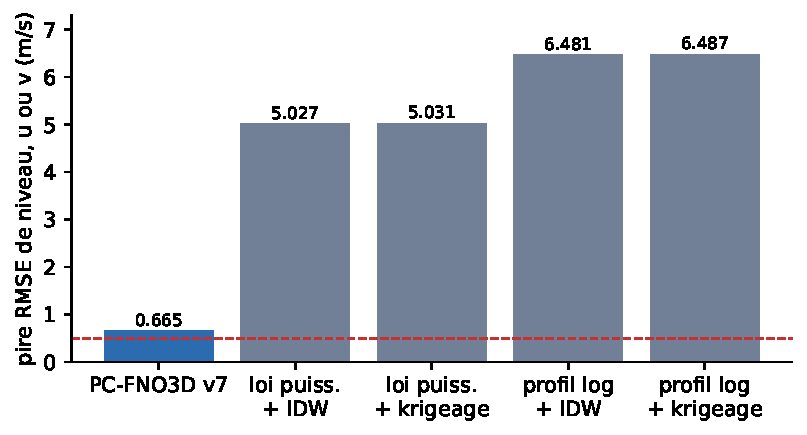
\includegraphics[width=0.85\linewidth]{figures/references_m8.pdf}
  \caption{Pire RMSE de niveau : PC-FNO3D contre les méthodes de référence (test synoptique).}
  \label{fig:references}
\end{figure}

L'erreur maximale de PC-FNO3D est 7,5 à 9,8 fois plus faible, et son $R^2$ minimal (0,991) est
loin devant celui des références (0,16 à 0,57). Trois études complémentaires du réseau ont été
menées :
\begin{itemize}
  \item \textbf{densité (E1)} : le modèle tient le DSO5 jusqu'à 50\,\% des capteurs ; aucune
        référence ne le tient, quelle que soit la densité ;
  \item \textbf{placement guidé par l'incertitude (E2)} : \textbf{résultat négatif} --- placer des
        capteurs là où l'incertitude est la plus forte fait pire que le hasard (2,39 contre
        1,28\ms) ;
  \item \textbf{capteur de secours (E3)} : sur ce réseau très dense, le krigeage (0,19\ms) remplace
        mieux un capteur en panne que la reconstruction 3D (1,50\ms).
\end{itemize}

\subsection{Fiabilité, alertes et éolien}
Pour la v7, la première lecture du DSO6 était non conforme (couverture de 75 à 81\,\%) ; une
seconde lecture, avec un facteur de calibration choisi sur la validation après ce premier verdict,
est conforme (87 à 91\,\%) mais n'est pas une mesure indépendante, et elle est publiée comme telle.
Le détecteur d'anomalies de capteurs (AN1) suit le même schéma : la v1 ne détectait que 5,2\,\% des
dérives ; la v2, fondée sur la cohérence avec les voisins et un modèle de site appris sur
l'entraînement, en détecte 100\,\% avec 2,2\,\% de fausses alertes (seconde lecture). Sur un parc
éolien de démonstration (3 éoliennes, 12\,MW), l'écart de production entre vent reconstruit et vent
vrai est de 1,71\,\% (seuil 5\,\%, EOL1).

\section{Domaine réel du Grand Tunis}

\subsection{Lignée des modèles}
\begin{figure}[H]
  \centering
  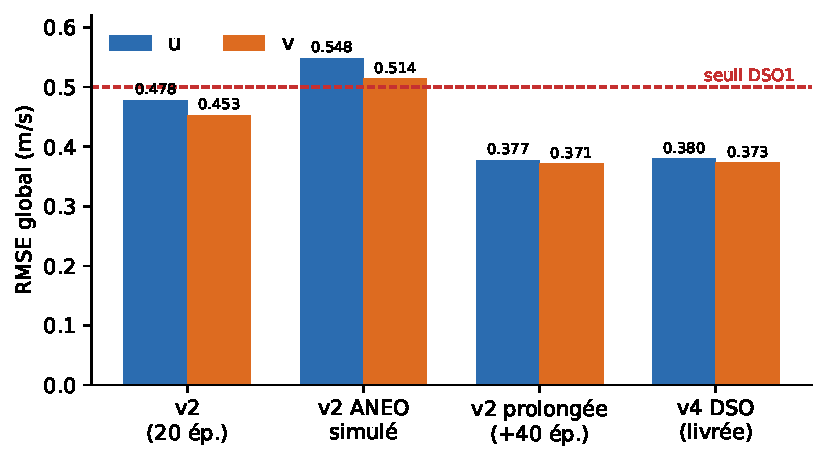
\includegraphics[width=0.85\linewidth]{figures/lignee_grand_tunis.pdf}
  \caption{RMSE global sur le test du Grand Tunis (180 instants) selon la version du modèle.}
  \label{fig:lignee}
\end{figure}

\begin{itemize}
  \item \textbf{v1} (champ entier, 25 canaux) : arrêtée à l'époque 14, $R^2$ de validation
        $u$ 0,78 / $v$ 0,73 ; le diagnostic montre que le profil ERA5 seul fait mieux (0,95 / 0,97) :
        il manque une entrée, ce n'est pas un défaut de code ;
  \item \textbf{v2} (34 canaux, correction d'ERA5, 20 époques) : $R^2$ de validation 0,986 / 0,992 ;
        test : RMSE global 0,478 / 0,453\ms, erreur de direction 3,9° ;
  \item \textbf{v2 ANEO simulé} (couche dense synthétique au lieu des stations) : moins bonne
        (0,548 / 0,514\ms) : une couche dense simulée n'apporte rien une fois le profil ERA5 en
        entrée ;
  \item \textbf{v2 prolongée} (+40 époques) : 0,377 / 0,371\ms, $R^2 \ge 0{,}98$ à tous les
        niveaux, erreur de direction 3,3° ; seul le niveau 25\,m reste au-dessus de 0,5\ms ;
  \item \textbf{v4} (affinage orienté DSO, $w$ par continuité) : livrée (section suivante).
\end{itemize}

\subsection{Décision de livraison de la v4}
La règle, écrite avant le test de la v4, était : la v4 n'est livrée que si elle n'est pas moins
bonne que la v2 prolongée sur DSO1, DSO4, DSO5 et les vraies mesures, avec une tolérance de 1\,\% et
aucune station dégradée de plus de 3\,\%. Le tableau~\ref{tab:v4} montre qu'elle l'est.

\begin{table}[H]
\centering
\caption{v4 (livrée) contre v2 prolongée, test du Grand Tunis (180 instants).}
\label{tab:v4}
\begin{tabularx}{\linewidth}{@{}Xccl@{}}
\toprule
Critère & v4 & v2 prolongée & Seuil\\
\midrule
RMSE global $u$ / $v$ (m/s) & 0,380 / 0,373 & 0,377 / 0,371 & ---\\
Pire RMSE de niveau (m/s) & 0,528 & 0,530 & $\le 0{,}5$\\
DSO2 ($w$ par continuité) & $1{,}05\cdot10^{-5}$ & $1{,}05\cdot10^{-5}$ & $\le 10^{-4}$\\
DSO4 (s) & 0,302 & 0,302 & $<1$\\
DSO5 25\,\% des entrées (m/s) & 0,535 & 0,537 & $\le 0{,}7$\\
Stations réelles, moyenne (m/s) & 2,469 & 2,467 & $\le$ v2 + 1\,\%\\
\bottomrule
\end{tabularx}
\end{table}

Sur la v4, le DSO6 est \textbf{conforme} dès la première lecture : couverture de l'intervalle à
80\,\% de 0,878 pour $u$, 0,883 pour $v$, 0,841 pour $w$ et 0,879 pour la vitesse, avec des
corrélations de Spearman positives (0,16 à 0,50) (figure~\ref{fig:dso6}).

\begin{figure}[H]
  \centering
  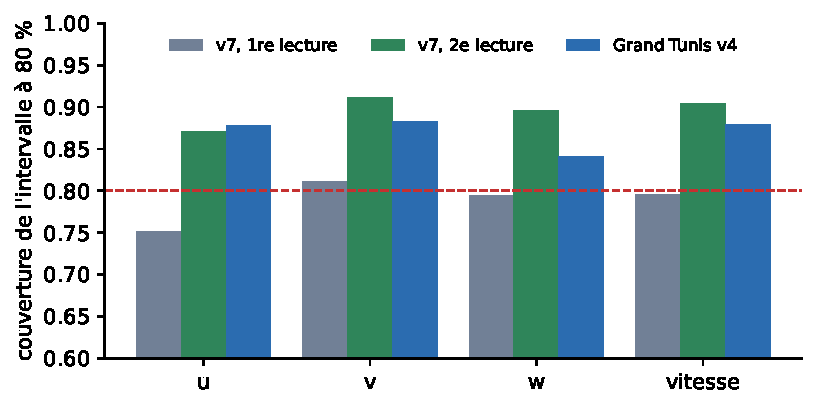
\includegraphics[width=0.82\linewidth]{figures/dso6_couverture.pdf}
  \caption{Couverture de l'intervalle à 80\,\% (DSO6).}
  \label{fig:dso6}
\end{figure}

\subsection{Validation sur les mesures réelles}
\begin{figure}[H]
  \centering
  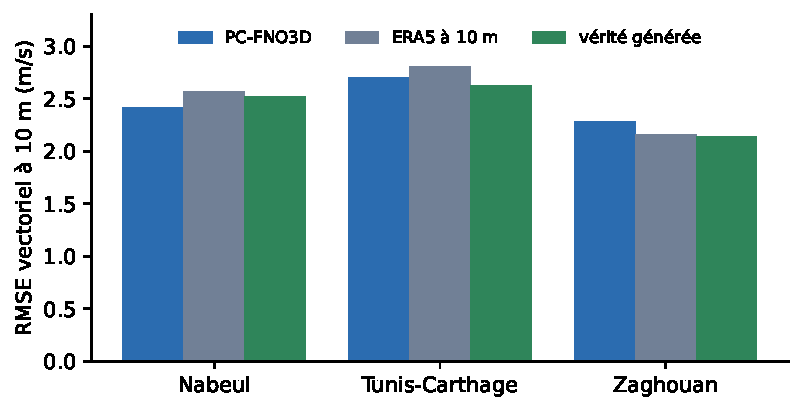
\includegraphics[width=0.82\linewidth]{figures/stations_reelles.pdf}
  \caption{Erreur aux stations réelles (station exclue de l'entrée), vent à 10\,m.}
  \label{fig:stations}
\end{figure}

Aux stations, le modèle est au niveau d'ERA5, un peu meilleur à Nabeul et Tunis-Carthage, un peu
moins bon à Zaghouan (figure~\ref{fig:stations}). Il reproduit la vérité générée, dont l'erreur
propre face aux stations est du même ordre : \emph{la limite est la vérité d'apprentissage, pas le
réseau}. Les erreurs de direction sont de 27 à 38° pour les trois sources, ce qui reflète la part
locale du vent qu'aucune n'explique. En altitude, sur les radiosondages de Tunis-Carthage (9 à 11
sondages par couche de 250\,m sur les blocs de test), le modèle fait mieux qu'ERA5 dans toutes les
couches de 0 à 1\,000\,m (RMSE vectoriel 1,95 à 2,34 contre 2,07 à 2,54\ms), avec un biais de
vitesse plus faible près du sol (0,58 contre 1,04\ms sous 250\,m).

\subsection{Affinage sur les stations : un gain illusoire}
La v3 a été affinée en prenant les trois stations comme cibles supplémentaires. Le modèle final
semblait spectaculaire à Tunis-Carthage et Zaghouan (figure~\ref{fig:v3}), mais moins bon à Nabeul,
où la station, abritée, mesure trop peu de vent. La \textbf{validation croisée spatiale}, où la
station jugée n'est jamais une cible, tranche : les gains tombent à $-1{,}5$, $-0{,}4$ et
$-0{,}5$\,\%, dans le bruit de mesure. La v3 a appris une \textbf{correction de site} aux points
cibles --- des taches de 0,8\ms dans le premier kilomètre autour des stations, moins de 0,1\ms au-delà
de 3\,km --- et non un meilleur champ entre les stations. La règle fixée à l'avance (gain moyen d'au
moins 5\,\% et d'au moins 3\,\% sur deux stations jamais vues) l'écarte, tout comme la variante v3b.

\begin{figure}[H]
  \centering
  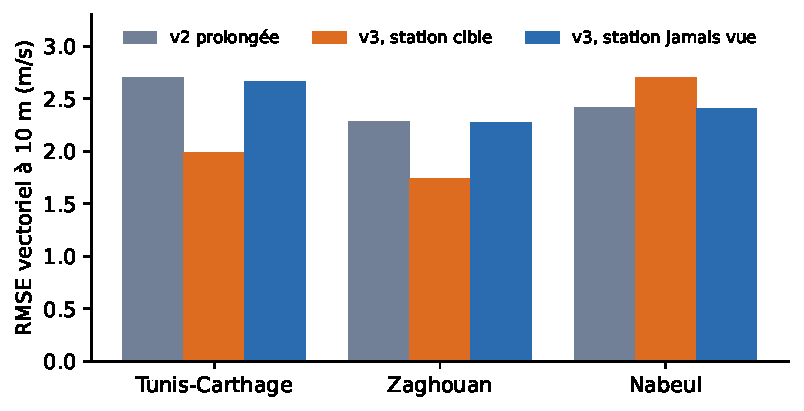
\includegraphics[width=0.82\linewidth]{figures/v3_validation_croisee.pdf}
  \caption{Affinage v3 : station cible contre station jamais vue (validation croisée spatiale).}
  \label{fig:v3}
\end{figure}

\section{Plan de déploiement du réseau ANEO (OS6)}
L'étude OS6 simule l'apport de capteurs ANEO : un capteur simulé est une maille où le modèle reçoit
la vérité de surface, comme une station réelle. 11\,890 emplacements candidats respectent les
contraintes (terre ferme, altitude au plus 650\,m, pente au plus 20°, 1\,km du bord et des autres
capteurs). Un placement glouton ajoute 5 capteurs par étape là où l'erreur résiduelle de validation
est la plus forte, jusqu'à 200 ; la courbe de dimensionnement compare ensuite, sur le test, le
placement optimisé, une grille régulière et des tirages au hasard (figure~\ref{fig:os6}).

\begin{figure}[H]
  \centering
  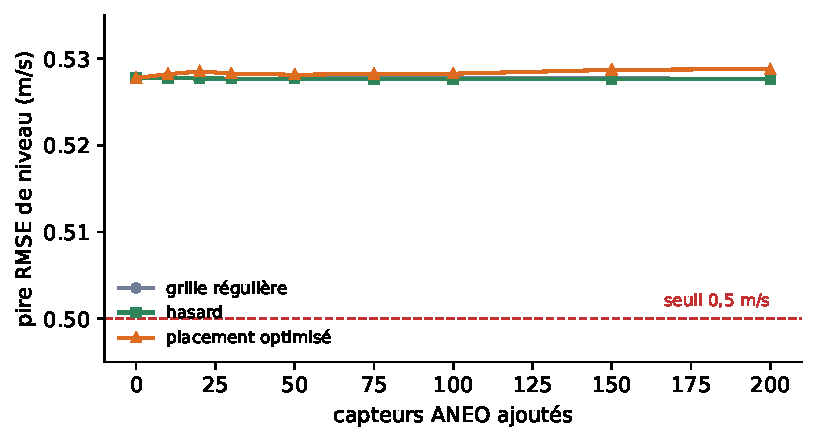
\includegraphics[width=0.82\linewidth]{figures/os6_courbe.pdf}
  \caption{OS6 : pire RMSE de niveau selon le nombre de capteurs ajoutés (test, 180 instants).}
  \label{fig:os6}
\end{figure}

Le résultat est \textbf{négatif} : de 10 à 200 capteurs, toutes les stratégies restent à
0,5326\ms de RMSE vectoriel et 0,528\ms au pire niveau, à $\pm0{,}0003$\ms près ; le placement
optimisé est même très légèrement moins bon. Aucun nombre de capteurs n'atteint le seuil (NET1 et
NET2 non conformes). Ce n'est pas un défaut de la simulation : les capteurs simulés reçoivent bien
la vraie valeur de surface. C'est une propriété du modèle livré : entraîné avec le treillis ERA5 et
trois stations, il s'appuie sur la grande échelle et traite une mesure ponctuelle comme une
correction locale. \textbf{Dimensionner le réseau demande un modèle entraîné à exploiter des
capteurs denses}, ce qui suppose un nouvel entraînement.

\section{Prévision à +24 et +48\,h (OS7)}
Le même modèle est nourri par la prévision GFS au lieu de la réanalyse. Les prévisions archivées
(NOAA, AWS) sont téléchargées pour chaque instant du cache aux échéances +24 et +48\,h (1\,000
échéances chacune), puis le modèle est affiné (v5) avec la même vérité et le même découpage, et
jugé sur 2022 contre GFS brut et la persistance (PREV1, PREV2), sur la décision de traitement de la
veille (PREV3) et sur les décisions agricoles aux stations (AGRI1, AGRI2).
\acompleter{Reporter ici les résultats d'OS7 (PREV1--3, AGRI1--2) une fois le calcul terminé.}

\section{Bilan de conformité}
Le bilan, produit automatiquement à partir des seuls résultats écrits, compte \textbf{18 critères
conformes, 4 non conformes, 1 proposé et 7 à mesurer} (tableau~\ref{tab:bilan}).

\begin{table}[H]
\centering
\caption{Bilan de conformité au cahier des charges (modèle livré v4).}
\label{tab:bilan}
\begin{tabularx}{\linewidth}{@{}lX@{}}
\toprule
Statut & Critères\\
\midrule
Conformes & DSO2, DSO4, DSO5, DSO6, REEL2, EOL2, DE1, DE2, DE3, PROD1, AN1 (seconde lecture), MCP1, API1, HIS1, EOL1 (parc de démonstration), REEL3, REEL4, NET2$^{*}$\\
Non conformes & DSO1 (0,528\ms au niveau 25\,m), DSO3 (0,805 : champ trop lisse), REEL1, NET1\\
Proposé & DSO7 (précision à densité réaliste, à fixer avec l'entreprise)\\
À mesurer & PREV1, PREV2, PREV3, AGRI1, AGRI2 (OS7), UX1, VIS1 (test utilisateur)\\
\bottomrule
\end{tabularx}
\par\smallskip\footnotesize $^{*}$ NET2 était compté conforme parce que la courbe existe ; la règle
corrigée exige aussi un nombre de capteurs suffisant, et NET2 est alors non conforme (5 non
conformes).
\end{table}

\section{Discussion}
Trois enseignements se dégagent.
\begin{enumerate}
  \item \textbf{La méthode fonctionne là où l'information existe} : sur le synthétique dense,
        PC-FNO3D surpasse largement les références et respecte la physique ; sur le réel, il
        améliore ERA5 en altitude et le vaut au sol.
  \item \textbf{La vérité d'apprentissage borne le résultat} : aux stations, le modèle ne peut pas
        faire mieux que le générateur qui lui sert de vérité ; les gains apparents d'un affinage
        sur les stations disparaissent dès qu'on juge sur des stations jamais vues.
  \item \textbf{Les règles fixées à l'avance ont évité trois fausses victoires} : la correction M1,
        l'affinage v3 et le placement guidé par l'incertitude auraient tous été retenus sur une
        lecture favorable du test.
\end{enumerate}
